% Typeset with XeTeX
% Allows use of system fonts rather than just LaTeX's ones
% NOTE - if you use TeXShop and Bibdesk (Mac), can complete citations
%  - open your .bib file, type~\citep{xx... and then F5 or Option-Escape
\documentclass[11pt]{article}
\usepackage[margin=1in, letterpaper]{geometry} % set page layout
%\geometry{letterpaper}  % or a4paper
\usepackage[xetex]{graphicx} % allows us to manipulate graphics.
% Replace option [] with pdftex if you don't use Xe(La)TeX
\usepackage{color}
\usepackage{indentfirst}
\usepackage{epstopdf} % automatic conversion of eps to pdf 
\usepackage{amsmath, amssymb} % Better maths support & more symbols
\usepackage{textcomp} % provide lots of new symbols - see textcomp.pdf
% line spacing: \doublespacing, \onehalfspacing, \singlespacing
\usepackage{setspace}
\singlespacing
\usepackage{pgfplotstable}
% allows text flowing around figs
% use \begin{wrapfigure}{x}{width} where x = r(ight) or l(eft)
\usepackage{wrapfig}
\usepackage[parfill]{parskip} % don't indent new paragraphs
\usepackage{flafter}  % Don't place figs & tables before their definition 
\usepackage{verbatim} % allows \begin and \end{comment} regions
\usepackage{booktabs} % makes tables look good
\usepackage{bm}  % Define \bm{} to use bold math fonts
% linenumbers in L margin, start & end with \linenumbers \nolinenumbers,
\usepackage{lineno} % use option [modulo] for steps of 5
\usepackage[auth-sc]{authblk} % authors & institutions - see authblk.pdf
%\renewcommand\Authands{ and } % separates the last 2 authors in the list
% control how captions look; here, use small font and indent both margins by 20pt
\usepackage[small]{caption} 
\setlength{\captionmargin}{20pt}

%: FONT
% If you don't want to use system fonts, replace from here to 'Citation style' with \usepackage{Palatino} or similar
%: ************ FANCY FONTS START HERE
\usepackage[no-math]{fontspec} % 'no-math' = keep computer modern for math fonts
\usepackage{xunicode} % needed by XeTeX for handling all the system fonts nicely
\usepackage[no-sscript]{xltxtra} 
\setmonofont[Scale=0.8]{PT Serif} % typeface for \tt commands
\setsansfont[BoldFont={PT Serif Bold}, ItalicFont={PT Serif Italic}]{PT Serif} 
\defaultfontfeatures{Mapping=tex-text}
%\setmainfont{Minion Pro}
\setmainfont{Source Sans Pro}

%: ************ FANCY FONTS END HERE

%:CITATION STYLE
% natbib package: square,curly, angle(brackets)
% colon (default), comma (to separate multiple citations)
% authoryear (default),numbers (citations style)
% super (for superscripted numerical citations, as in Nature)
% sort (orders multiple cites into order of appearance in ref list, or year if authoryear)
% sort&compress: as sort, + multiple citations compressed (as 3-6, 15)
\usepackage[numbers,comma,sort&compress]{natbib}

%:SHORTCUT COMMANDS
% Maths
\newcommand{\ddt}[1]{\ensuremath{\frac{{\rm d}#1}{{\rm d}t}}}  % d/dt
\newcommand{\dd}[2]{\ensuremath{\frac{{\rm d}#1}{{\rm d}#2}}} % dy by dx  - \dd{y}{x}
\newcommand{\ddsq}[2]{\ensuremath{\frac{{\rm d}^2#1}{{\rm d}#2^2}}} % second deriv
\newcommand{\pp}[2]{\ensuremath{\frac{\partial #1}{\partial #2}}} % partial \pp{y}{x}
\newcommand{\ppsq}[2]{\ensuremath{\frac{\partial^2 #1}{\partial {#2}^2}}}
\newcommand{\superscript}[1]{\ensuremath{^{\textrm{#1}}}} %normal (non-math) font for super/subscripts in text
\newcommand{\subscript}[1]{\ensuremath{_{\textrm{#1}}}}
\newcommand{\positive}{\ensuremath{^+}}
\newcommand{\negative}{\ensuremath{^-}}
% Editing
\newcommand{\red}[1]{{\color{red}{#1}}}
\newcommand{\redtext}[1]{{\color{red}{#1}}}
\newcommand{\blue}[1]{{\color{blue}{#1}}}
\newcommand{\bluetext}[1]{{\color{blue}{#1}}}
\newcommand{\scinot}[2]{\ensuremath{#1 \times 10^{#2}}}
% Standard stuff
\newcommand{\be}{\begin{equation}}
\newcommand{\ee}{\end{equation}}
\newcommand{\bea}{\begin{eqnarray}}
\newcommand{\eea}{\end{eqnarray}}
\newcommand{\ie}{\textit{i.e.}}
\newcommand{\etal}{\textit{et al.}}
\newcommand{\khi}{Ki67$^\text{hi}$}
\newcommand{\klo}{Ki67$^\text{lo}$}


% \begin{graybox} text \end{graybox} for text with a background colour
\definecolor{MyGray}{rgb}{0.96,0.97,0.98}
\definecolor{MyGray}{rgb}{0.96,0.90,0.98}
\makeatletter\newenvironment{graybox}{%
	\begin{lrbox}
	{\@tempboxa}\begin{minipage}[r]{0.98\columnwidth}}{\end{minipage}\end{lrbox}%
	\colorbox{MyGray}{\usebox{\@tempboxa}}
}\makeatother


%%%%%%%%%%%%%%%%%%%%%%%

\title{Issues with MZ model fits and ki67 predictions}
\author{}

\date{}

\begin{document} 
\maketitle

\begin{itemize}
	\item \textbf{T2 as the source} : The kinetics of total cell counts and normalised donor frations (f$_\text{d}$) of MZ cells are best exlplained by the age-structured model ($\Delta \text{AIC} = 3$, Table~\ref{tab:MZs_extended}, also Figure\ref{fig:ASM_MZ} A).
	Fails to explain the timecourse of \khi fractions (Figure\ref{fig:ASM_MZ} B).
	
	\item \textbf{T1 as the source} : Most support for the time-dependent model ($\Delta \text{AIC} = 9$, Table~\ref{tab:MZs_extended}, also Figure\ref{fig:TDM_MZ} A).
	Also, fails to explain the timecourse of \khi fractions (Figure\ref{fig:TDM_MZ} B).
	
	\item All the other models followed the same trend $\rightarrow$ Failed to capture the kinetics of \khi fractions using parameters estimated from the fits to cell counts and f$_\text{d}$.
	
	\item Varying the rate of source influx in all the models mentioned in table~\ref{tab:MZs_extended}, does not improve their ability to predict the kinetics of \khi fractions.
	
	\item We tried combination of different models. The hybrid models were over-parametrised (the algorithm that we use to fit models may run into problems for more than 5 unknown parameters). Therefore, we decided to run simulations of cell counts, f$_\text{d}$ and ki67 kinetics and fixed some of the parameters before fitting these models to the data.
	
	\item The time-dependent + incumbent combination shows the best compromise between model fits to the cell counts and f$_\text{d}$ and the predictions of \khi fractions (Figure~\ref{fig:TDM_INC_MZ} A and B). These fits were generated using T2 as the source and the rate of source influx was fixed based on the simulations. I also had to assume that the fraction of \khi cells in source influx `$\epsilon$' to be 1 in order to generate ki67 predictions.
	
	\item We are not happy with these fits and hence trying few other models. Since, cell counts of MZ cells seem to be tightly regulated, tried density-dependent model $\rightarrow$ didn't work. Currently, testing density-dependent model in combination with other models. No luck so far.
	
	\item Melissa provided some interesting information about age-associated B cells (ABCs) contaminating the MZ compartment. This might explain all the troubles we are facing with MZ cells. 
	
	\item If there is a contaminating population of ABCs with different dynamics in the MZ compartment then the kinetic heterogeneity (KH) model should be able to explain the data. However, KH model fails to capture the trend in ki67 $\rightarrow$ probably because of the time-dependent kinetics of accumulation of ABCs at the marginal zone. I think ABCs are folicular cells that lose their complement receptor (CD21) expression (probably due to exhaustion) and migrate to the marginal zone since they cant compete for folicular retention without CD21. [Michael caroll, Seminars in Imm. August 1998]
	
	\item The time-dependent effects in \khi fractions in the donor MZ population can be explained by gradual migration of \klo ABCs into the MZ pool. The big assumption here is that MZ cells have high \khi fractions due to frequent divisions. 
	
	
\end{itemize}



%: Table 1.2
\begin{table}[h!]
	\small{
		\begin{center}
			\renewcommand{\arraystretch}{1.25}
			\begin{tabular}{ l | m{1.2cm} | c | m{2cm} | m{2cm} | m{2cm} | m{2cm} | m{2cm}} 
				\toprule[0.05cm]
				\textbf{Model} & \textbf{Source}  & \textbf{$\Delta$AIC} & \textbf{Mean residence time $\tau$ (d)}  & \textbf{Time taken for $\tau$ to double (d)}  & \textbf{Mean inter-division time (d)} & \textbf{Mean clonal life-time (d) for subset1} & \textbf{Mean clonal life-time(d) for subset2} \\
				\hline
				Time-dependent & T1 & 0   & 19(7, 55)  & 800(240, 2600)  & 28(7, 120)  &  --  & -- \\
				               & T2 & 34  & 32(11, 90) & 810(200,3200)   & 64(9,460)   &  --  & -- \\  
				\hline
				Age-structured & T1 & 9    & 9(5, 16)  & 1100(590, 2100)  & 11(5, 22)  &  --  & -- \\
				               & T2 & 31   & 11(5, 23) & 630(270, 1400)   & 15(6, 38)  &  --  & -- \\  
				\hline
				Simple         & T1 & 12   & -- & --  &  -- & 111 (142, 100)  & -- \\
				birth-death    & T2 & 36   & -- & --  &  -- & 90 (66, 125)    & -- \\  
				\hline
				Incumbent      & T1 & 11   & -- & --  &  -- & 103(73, 171)    & -- \\
				               & T2 & 35   & -- & --  &  -- & 67(45, 125)     & -- \\  
				\hline
				Kinetic        & T1 & 8    & -- & --  &  -- & 270(106, 710)   & 73(52, 102)  \\
				heterogeneity  & T2 & 34   & -- & --  &  -- & 170(34, 840)    & 63(18, 210)  \\  
				\hline
				\toprule 
			\end{tabular}
		\end{center}
		\caption{\small \textbf{Comparison of AIC values and parameter estimates using either T1 or T2 as the source population from different models fitted to cell counts and donor fractions$^{\dagger}$ in MZ B cells.}}
		$^{\dagger}$ \footnotesize For the incumbent, kinetic heterogeneity and simple birth-death model we only have $\lambda$ estimates. \\
		$^\ast$ \footnotesize r is the rate of change of residence-time with host-age or cell age, hence log(2)/r denotes the average time taken for mean residence time `$\tau$' to double. \\ Changing $\rho$ with time or cell age gives (visually) poor fits hence not included in this analysis. \\
		\label{tab:MZs_extended}
	}
\end{table} 


\begin{figure}[h!]
	\centerline{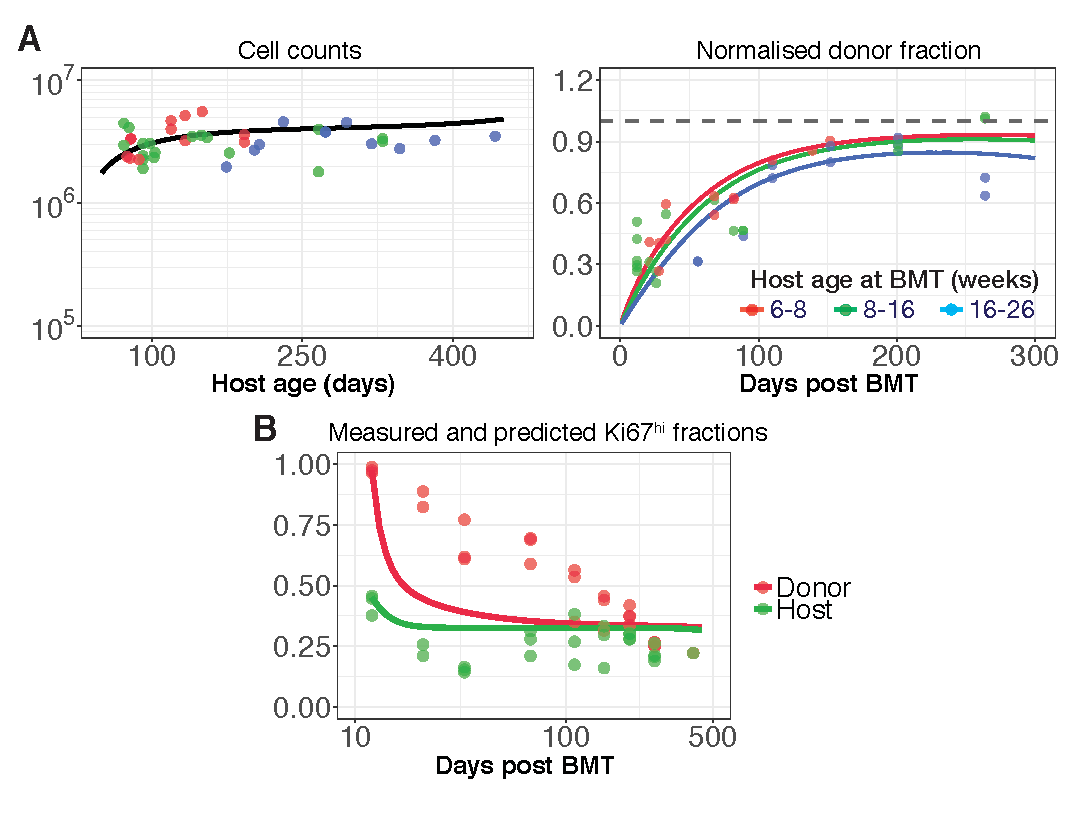
\includegraphics[scale = 0.85] {ASM_MZ.pdf}}
	\caption{\small \textbf{Fitted and predicted   population dynamics of MZ B cells, using the age-structure model in which the mean residence time of cell increases with their age.}  (A) The model was fitted simultaneously to the extended timecourses of total cell counts and the donor fractions in MZ B cells normalised to the chimerism in T2 cells. The latter took account of different ages at BMT (right-hand panel, coloured lines; each generated using the  mode of the age within each group). (B) We then used the model parameters to predict the proportion of cells that were \khi\ within host and donor MZ B cells over time.}
	\label{fig:ASM_MZ}
\end{figure}

\begin{figure}[h!]
	\centerline{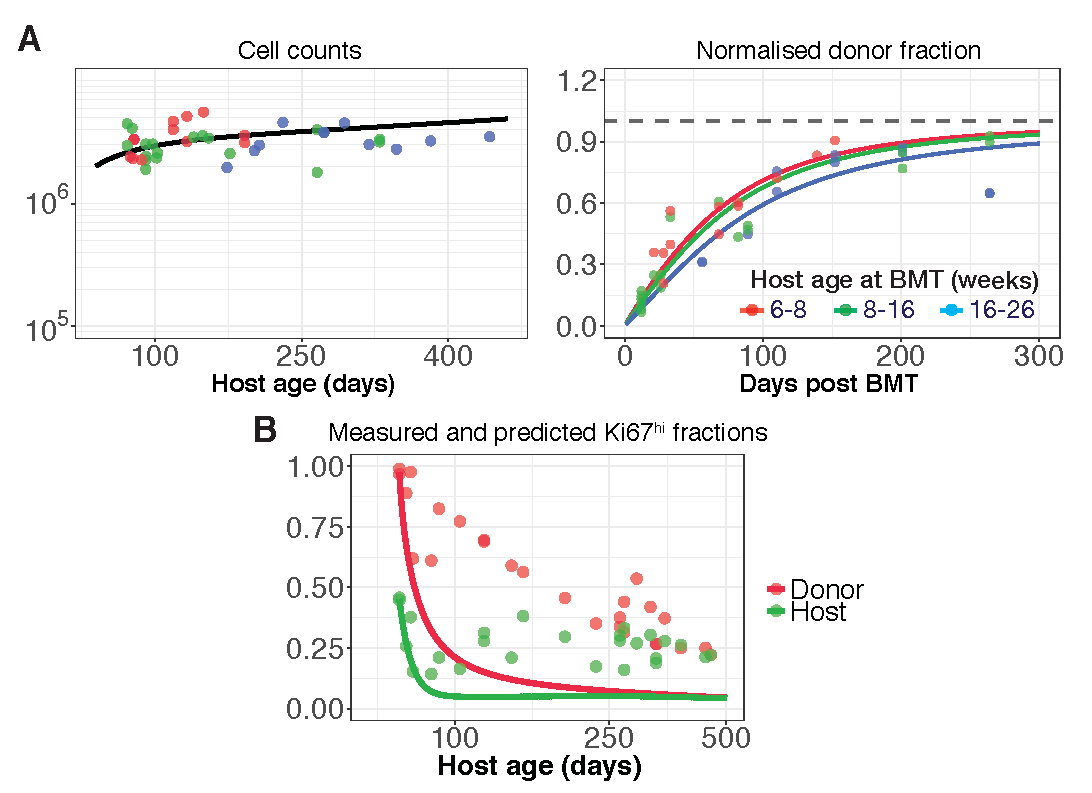
\includegraphics[scale = 0.85] {TDM_MZ.pdf}}
	\caption{\small \textbf{Fitted and predicted population dynamics of MZ B cells, using the time-dependent model in which the mean residence time of cell increases with the age of the host.}  (A) The model was fitted simultaneously to the extended timecourses of total cell counts and the donor fractions in MZ B cells normalised to the chimerism in T1 cells. The latter took account of different ages at BMT (right-hand panel, coloured lines; each generated using the  mode of the age within each group). (B) We then used the model parameters to predict the proportion of cells that were \khi\ within host and donor MZ B cells over time.}
	\label{fig:TDM_MZ}
\end{figure}


\begin{figure}[h!]
	\centerline{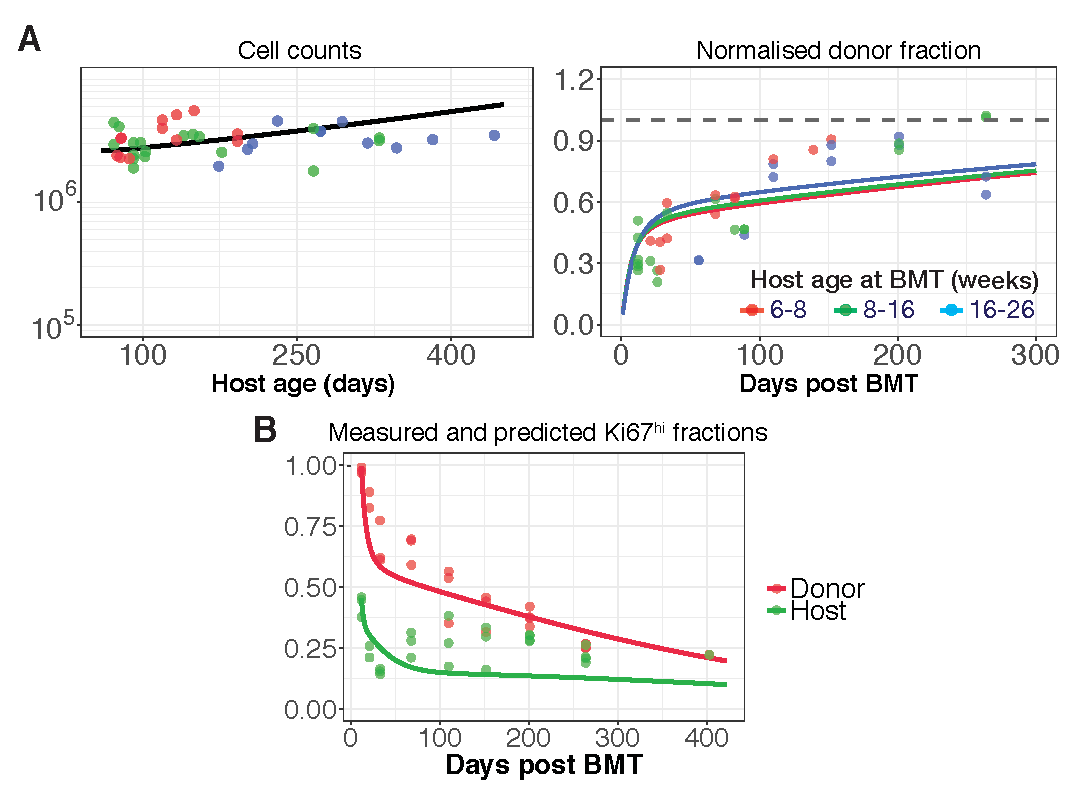
\includegraphics[scale = 0.85] {TDM_INC_MZ.pdf}}
	\caption{\small \textbf{Fitted and predicted population dynamics of MZ B cells, using the time-dependent +incumbent hybrid model.}  (A) The model was fitted simultaneously to the extended timecourses of total cell counts and the donor fractions in MZ B cells normalised to the chimerism in T2 cells. The latter took account of different ages at BMT (right-hand panel, coloured lines; each generated using the  mode of the age within each group). (B) We then used the model parameters to predict the proportion of cells that were \khi\ within host and donor MZ B cells over time.}
	\label{fig:TDM_INC_MZ}
\end{figure}



\end{document}